%%%%%%%%%%%%%%%%%%%%%%%%%%%%%%%%%%%%%%%%%%%%%%%%%%
\section{Introduction}
\label{sec:introduction}
%%%%%%%%%%%%%%%%%%%%%%%%%%%%%%%%%%%%%%%%%%%%%%%%%%

%-------------
The standard model (SM) of fundamental particles and their interactions has been extremely successful in describing phenomena in the atomic and subatomic realms.
%
After the discovery of a boson with properties consistent with the SM Higgs at the LHC~\cite{Chatrchyan:2012ufa,Aad:2012tfa}, attention has shifted to searches for new physics to explain the fine-tuned cancellation of large quantum corrections required  to stabilize the Higgs boson at a light mass of 125~GeV~\cite{finetune1,finetune2,finetune3,finetune4,finetune5,finetune5,finetune6}. 
%
Supersymmetry (SUSY) is a new symmetry beyond the SM that provides an elegant mechanism to mitigate this hierarchy problem.
%
SUSY proposes a super-partner for each SM particle with the same quantum numbers except for spin, which differs by a half-integer unit.
%
The loop corrections to the Higgs boson mass due to these sparticles are opposite in sign to those of the SM particles~\cite{Barbieri:1987fn,deCarlos1993320,Dimopoulos1995573,Barbieri199676,Papucci:2011wy} predicting a finite value for the Higgs boson mass.
%
This behavior can survive the breaking of SUSY, which is necessary to explain the non-observation of superpartners with exactly the same mass as their SM counterparts, provided that the superpartners are not themselves too heavy.
%
In addition to solving the problem of radiative stability, some SUSY models also offer a dark matter candidate to explain astrophysical observations~\cite{DarkMatterReview,DMGeneral}.

%-------------
Of particular interest is the search for the top squark, the SUSY partner of the top quark, which should be relatively light (less than $\sim 1\TeV$) for SUSY to provide a natural, rather than fine-tuned, solution to the hierarchy problem. 
%
Searches for top squark pair production have been performed by the ATLAS Collaboration~\cite{ATLAS1,ATLAS2,ATLAS5,ATLAS5a,ATLAS6,ATLAS7,ATLAS8} and the CMS Collaboration~\cite{CMS-STOP-had,CMS-STOP-lepton,CMS-alphaT,CMS-tophiggsino,CMS-SUS-13-024,CMS-SUS-14-010,RAZOR_8TeV,stop8TeV,hadstop_UCSB} at the LHC using the Run~1 data.
%
This summary reports on a search for top squark production in multijet events with a large imbalance in transverse momentum, based on 13~TeV data collected by the CMS experiment in 2015.
%
The search strategy follows closely the one reported in~\cite{stop8TeV} with several improvements. 
%
For this search, the top squark mass is assumed to be sufficiently large such that the decay into a top quark is always available. 
%
We then study two decay branching fraction scenarios: first, when a top squark decays with 100\% probability to a top quark and a stable, weakly interacting, lightest neutralino $\sTop\rightarrow\topquark\chiOneZero$, referred to as the T2tt model; and second, when a top squark decays with 50\% probability to a bottom quark and the lightest chargino $\sTop\rightarrow\bottomquark\chiOnePlus$ (which subsequently decays to a virtual W boson and the $\chiOneZero$), referred to as the T2tb model. 
%
The T2tb model assumes a gaugino mass splitting between the \chiOnePlus and the \chiOneZero of 5~GeV.
%
The main target signal processes of top squark pair production considered in this search are represented pictorially in Figure~\ref{Fig:signal_diagrams}.

%-------------
A central feature of the analysis is the use of a novel top quark tagging algorithm inspired by the one described in~\cite{Kaplan:2008ie,Plehn:2010st,Kaplan:2012gd} for increased signal-to-background sensitivity.
%
This top quark tagging algorithm is improved, with respect to the one described in Ref.~\cite{stop8TeV}, to enhance the sensitivity for top quark decays where either the W boson or the products of the entire top quark decay mostly merge into a single jet, as expected for highly-boosted top quarks.
%
The analysis is based on exclusive search regions defined in terms of the number of top quark candidates and the number of b-tagged jets, as well as the value of missing momentum (\MET) and \MTTwo.
%
The background estimation follows well-established methods, mostly data driven, that have been used in previous CMS analyses~\cite{RA2,RA2_2011,RA2_2012,stop8TeV}.

%%%%%%%%%%%%%%%%%%%%%%%%%%%%%%%%%%%%%%%%%%%%%%%%%%
\begin{figure}[ht!]
\begin{centering}
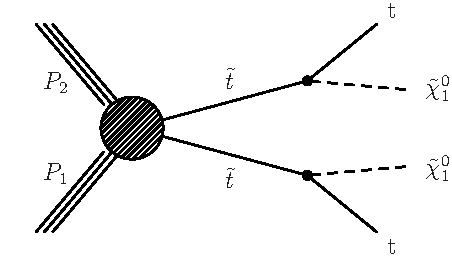
\includegraphics[width=0.40\textwidth]{figures/T2tt.pdf}
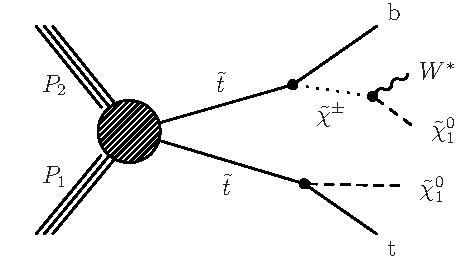
\includegraphics[width=0.40\textwidth]{figures/T2tb.pdf}\\
\caption{Signal models of interest in this search: 
top squark pair production with the top squark decaying into a top quark and 
neutralino or into a bottom quark and chargino.} 
\label{Fig:signal_diagrams}
\end{centering}
\end{figure}
%%%%%%%%%%%%%%%%%%%%%%%%%%%%%%%%%%%%%%%%%%%%%%%%%%
